% xcolor and define colors -------------------------
\usepackage{xcolor}

% https://www.viget.com/articles/color-contrast/
\definecolor{purple}{HTML}{5601A4}
\definecolor{navy}{HTML}{0D3D56}
\definecolor{ruby}{HTML}{9a2515}
\definecolor{alice}{HTML}{107895}
\definecolor{daisy}{HTML}{EBC944}
\definecolor{coral}{HTML}{F26D21}
\definecolor{kelly}{HTML}{829356}
\definecolor{cranberry}{HTML}{E64173}
\definecolor{jet}{HTML}{131516}
\definecolor{asher}{HTML}{555F61}
\definecolor{slate}{HTML}{314F4F}

% Mixtape Sessions
\definecolor{picton-blue}{HTML}{00b7ff}
\definecolor{violet-red}{HTML}{ff3881}
\definecolor{sun}{HTML}{ffaf18}
\definecolor{electric-violet}{HTML}{871EFF}

\newcommand\pictonBlue[1]{{\color{picton-blue}#1}}
\newcommand\sun[1]{{\color{sun}#1}}
\newcommand\electricViolet[1]{{\color{electric-violet}#1}}
\newcommand\violetRed[1]{{\color{violet-red}#1}}

\newcommand\bgPictonBlue[1]{{\colorbox{picton-blue!20!white}{#1}}}
\newcommand\bgSun[1]{{\colorbox{sun!20!white}{#1}}}
\newcommand\bgElectricViolet[1]{{\colorbox{electric-violet!20!white}{#1}}}
\newcommand\bgVioletRed[1]{{\colorbox{violet-red!20!white}{#1}}}

\def\code#1{\texttt{#1}}

% Main theme colors
\definecolor{accent}{HTML}{00b7ff}
\definecolor{accent2}{HTML}{871EFF}
\definecolor{gray100}{HTML}{f3f4f6}
\definecolor{gray800}{HTML}{1F292D}


% Beamer Options -------------------------------------

% Background
\setbeamercolor{background canvas}{bg = white}

% Change text margins
\setbeamersize{text margin left = 15pt, text margin right = 15pt} 

% \alert
\setbeamercolor{alerted text}{fg = accent2}

% Frame title
\setbeamercolor{frametitle}{bg = white, fg = jet}
\setbeamercolor{framesubtitle}{bg = white, fg = accent}
\setbeamerfont{framesubtitle}{size = \small, shape = \itshape}

% Block
\setbeamercolor{block title}{fg = white, bg = accent2}
\setbeamercolor{block body}{fg = gray800, bg = gray100}

% Title page
\setbeamercolor{title}{fg = gray800}
\setbeamercolor{subtitle}{fg = accent}

%% Custom \maketitle and \titlepage
\setbeamertemplate{title page}
{
    %\begin{centering}
        \vspace{20mm}
        {\Large \usebeamerfont{title}\usebeamercolor[fg]{title}\inserttitle}\\
        {\large \itshape \usebeamerfont{subtitle}\usebeamercolor[fg]{subtitle}\insertsubtitle}\\ \vspace{10mm}
        {\insertauthor}\\
        {\color{asher}\small{\insertdate}}\\
    %\end{centering}
}

% Table of Contents
\setbeamercolor{section in toc}{fg = accent!70!jet}
\setbeamercolor{subsection in toc}{fg = jet}

% Button 
\setbeamercolor{button}{bg = accent}

% Remove navigation symbols
\setbeamertemplate{navigation symbols}{}

% Table and Figure captions
\setbeamercolor{caption}{fg=jet!70!white}
\setbeamercolor{caption name}{fg=jet}
\setbeamerfont{caption name}{shape = \itshape}

% Bullet points

%% Fix spacing between items
\let\olditemize=\itemize 
\let\endolditemize=\enditemize 
\renewenvironment{itemize}{\vspace{0.25em}\olditemize \itemsep0.25em}{\endolditemize}

%% Fix left-margins
\settowidth{\leftmargini}{\usebeamertemplate{itemize item}}
\addtolength{\leftmargini}{\labelsep}

%% enumerate item color
\setbeamercolor{enumerate item}{fg = accent}
\setbeamerfont{enumerate item}{size = \small}
\setbeamertemplate{enumerate item}{\insertenumlabel.}

%% itemize
\setbeamercolor{itemize item}{fg = accent!70!white}
\setbeamerfont{itemize item}{size = \small}
\setbeamertemplate{itemize item}[circle]

%% right arrow for subitems
\setbeamercolor{itemize subitem}{fg = accent!60!white}
\setbeamerfont{itemize subitem}{size = \small}
\setbeamertemplate{itemize subitem}{$\rightarrow$}

\setbeamertemplate{itemize subsubitem}[square]
\setbeamercolor{itemize subsubitem}{fg = jet}
\setbeamerfont{itemize subsubitem}{size = \small}








% Links ----------------------------------------------

\usepackage{hyperref}
\hypersetup{
  colorlinks = true,
  linkcolor = accent2,
  filecolor = accent2,
  urlcolor = accent2,
  citecolor = accent2,
}


% Line spacing --------------------------------------
\usepackage{setspace}
\setstretch{1.35}


% \begin{columns} -----------------------------------
\usepackage{multicol}


% Fonts ---------------------------------------------
% Beamer Option to use custom fonts
\usefonttheme{professionalfonts}

% \usepackage[utopia, smallerops, varg]{newtxmath}
% \usepackage{utopia}
\usepackage[sfdefault,light]{roboto}

% Small adjustments to text kerning
\usepackage{microtype}



% Remove annoying over-full box warnings -----------
\vfuzz2pt 
\hfuzz2pt


% Table of Contents with Sections
\setbeamerfont{myTOC}{series=\bfseries, size=\Large}
\AtBeginSection[]{
        \frame{
            \frametitle{Roadmap}
            \tableofcontents[current]   
        }
    }


% Tables -------------------------------------------
% Tables too big
% \begin{adjustbox}{width = 1.2\textwidth, center}
\usepackage{adjustbox}
\usepackage{array}
\usepackage{threeparttable, booktabs, adjustbox}
    
% Fix \input with tables
% \input fails when \\ is at end of external .tex file
\makeatletter
\let\input\@@input
\makeatother

% Tables too narrow
% \begin{tabularx}{\linewidth}{cols}
% col-types: X - center, L - left, R -right
% Relative scale: >{\hsize=.8\hsize}X/L/R
\usepackage{tabularx}
\newcolumntype{L}{>{\raggedright\arraybackslash}X}
\newcolumntype{R}{>{\raggedleft\arraybackslash}X}
\newcolumntype{C}{>{\centering\arraybackslash}X}

% Figures

% \imageframe{img_name} -----------------------------
% from https://github.com/mattjetwell/cousteau
\newcommand{\imageframe}[1]{%
    \begin{frame}[plain]
        \begin{tikzpicture}[remember picture, overlay]
            \node[at = (current page.center), xshift = 0cm] (cover) {%
                \includegraphics[keepaspectratio, width=\paperwidth, height=\paperheight]{#1}
            };
        \end{tikzpicture}
    \end{frame}%
}

% subfigures
\usepackage{subfigure}


% Highlight slide -----------------------------------
% \begin{transitionframe} Text \end{transitionframe}
% from paulgp's beamer tips
\newenvironment{transitionframe}{
    \setbeamercolor{background canvas}{bg=accent!40!black}
    \begin{frame}\color{accent!10!white}\LARGE\centering
}{
    \end{frame}
}


% Table Highlighting --------------------------------
% Create top-left and bottom-right markets in tabular cells with a unique matching id and these commands will outline those cells
\usepackage[beamer,customcolors]{hf-tikz}
\usetikzlibrary{calc}
\usetikzlibrary{fit,shapes.misc}

% To set the hypothesis highlighting boxes red.
\newcommand\marktopleft[1]{%
    \tikz[overlay,remember picture] 
        \node (marker-#1-a) at (0,1.5ex) {};%
}
\newcommand\markbottomright[1]{%
    \tikz[overlay,remember picture] 
        \node (marker-#1-b) at (0,0) {};%
    \tikz[accent!80!jet, ultra thick, overlay, remember picture, inner sep=4pt]
        \node[draw, rectangle, fit=(marker-#1-a.center) (marker-#1-b.center)] {};%
}


% DAGS ----------------------------------------------
\usepackage{tikz}
\usetikzlibrary{shapes,decorations,arrows,calc,arrows.meta,fit,positioning}
% Tikz settings optimized for causal graphs.
\tikzset{
    -Latex,auto,node distance =1 cm and 1 cm,semithick,
    state/.style ={ellipse, draw, minimum width = 0.7 cm},
    point/.style = {circle, draw, inner sep=0.04cm,fill,node contents={}},
    bidirected/.style={Latex-Latex,dashed},
    el/.style = {inner sep=2pt, align=left, sloped}
}


% Beamer tricks -------------------------------------
% Make \pause work in align environments
\makeatletter
\renewrobustcmd{\beamer@@pause}[1][]{%
  \unless\ifmeasuring@%
  \ifblank{#1}%
    {\stepcounter{beamerpauses}}%
    {\setcounter{beamerpauses}{#1}}%
  \onslide<\value{beamerpauses}->\relax%
  \fi%
}
\makeatother


\begin{document}
\title{Quasi Experimental Methods}
\author{Chris Conlon}
\institute{NYU Stern}
\date{\today}

\frame{\titlepage}


\begin{frame}{}
\begin{itemize}
\item What about an actual experiment that someone else ran?
\item Something that isn’t an experiment but sort of looks like one?
\item We want \alert{as good as random} variation.
\end{itemize}
\end{frame}
\section{Lotteries}

\begin{frame}{Angrist, Pathak, Walters (2013)}
Are charter schools effective at improving educational outcomes?
\begin{itemize}
    \item Challenge: Simply being willing to sign up for a Charter school may mean you care more about education than the average student.\\
    This is the \alert{selection problem}.
    \item Solution: Charters are over-subscribed, more students sign up that can be accomodated, and a lottery is held.
    \item Compare students who win the lottery to those that lose the lottery but otherwise look similar.
\end{itemize}
\end{frame}



\begin{frame}{Angrist, Pathak, Walters (2013)}
\begin{figure}
\centering
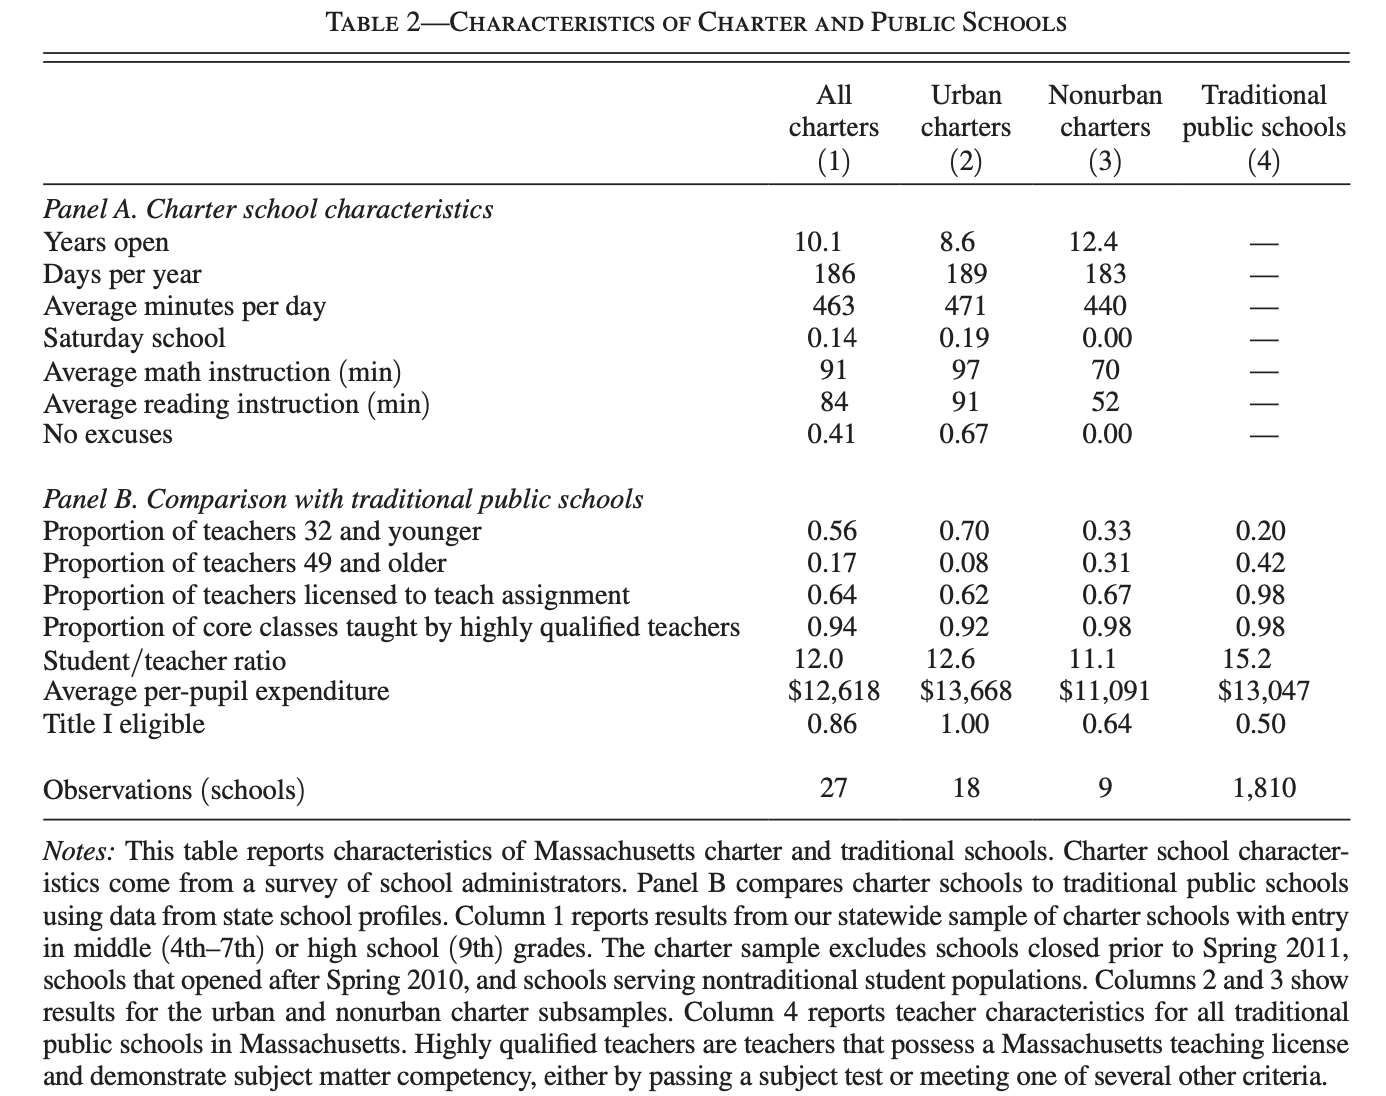
\includegraphics[width=4.5in]{./resources/apw_1.png}
\end{figure}
\end{frame}

\begin{frame}{Angrist, Pathak, Walters (2013)}
\begin{figure}
\centering
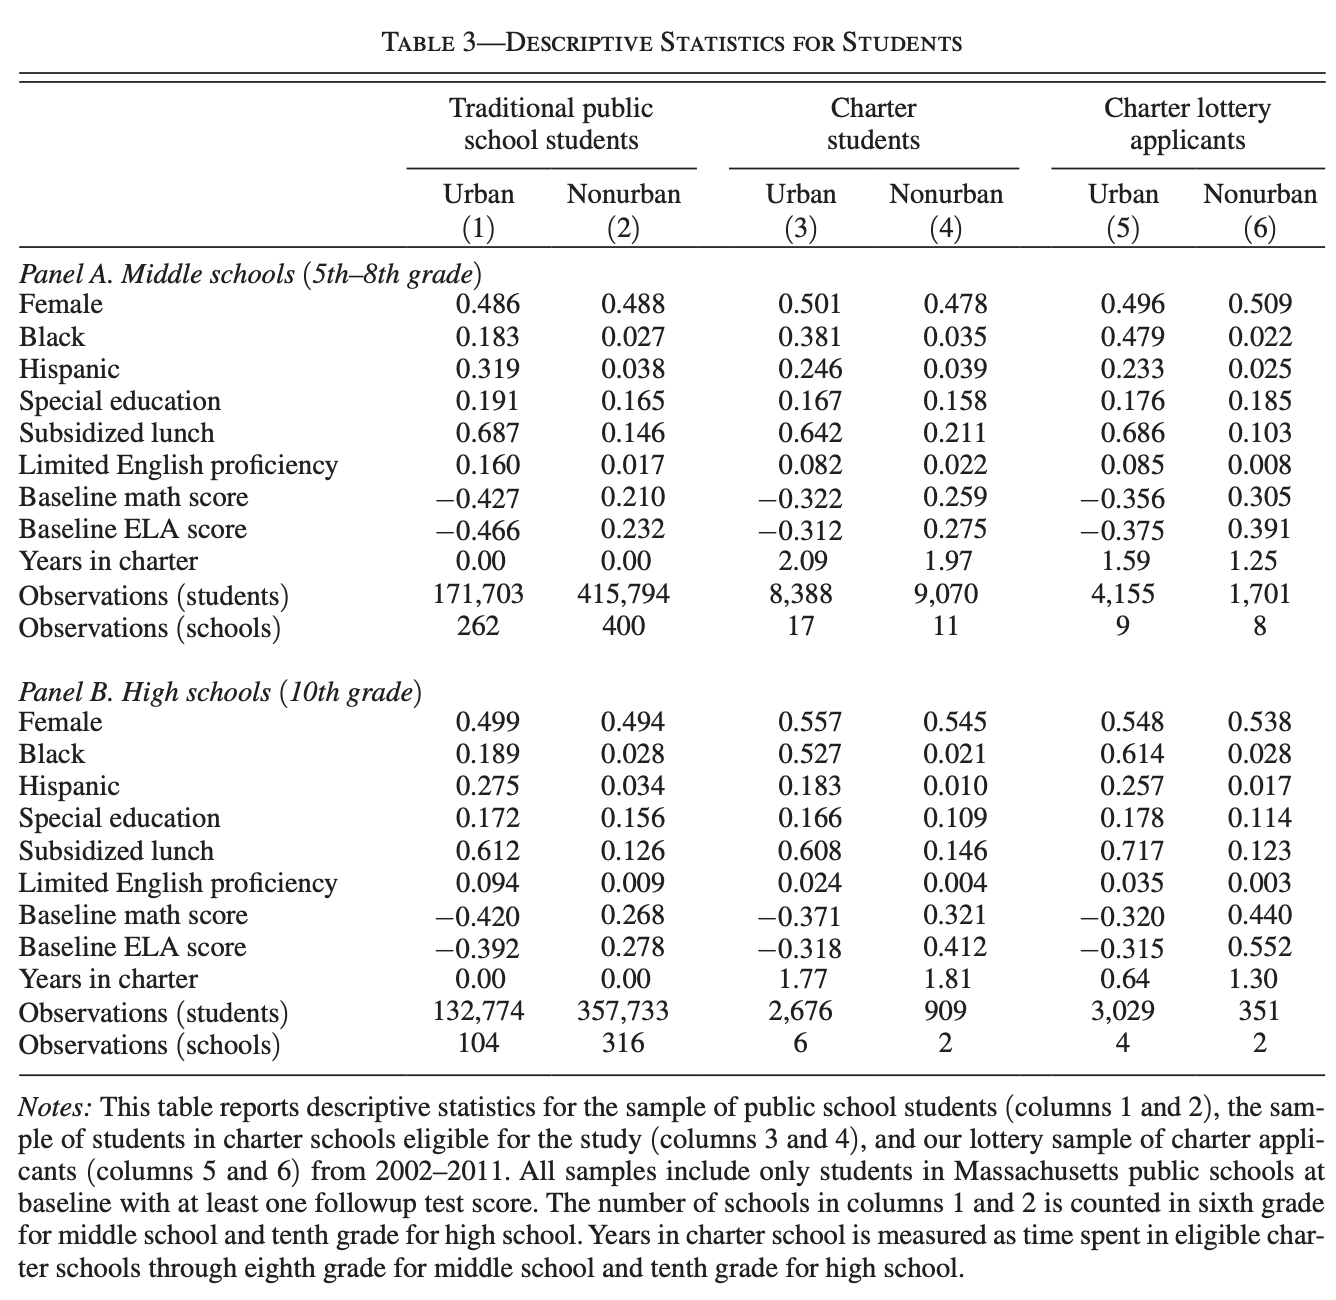
\includegraphics[width=3.5in]{./resources/apw_2.png}
\end{figure}
\end{frame}

\begin{frame}{Angrist, Pathak, Walters (2013)}
\begin{figure}
\centering
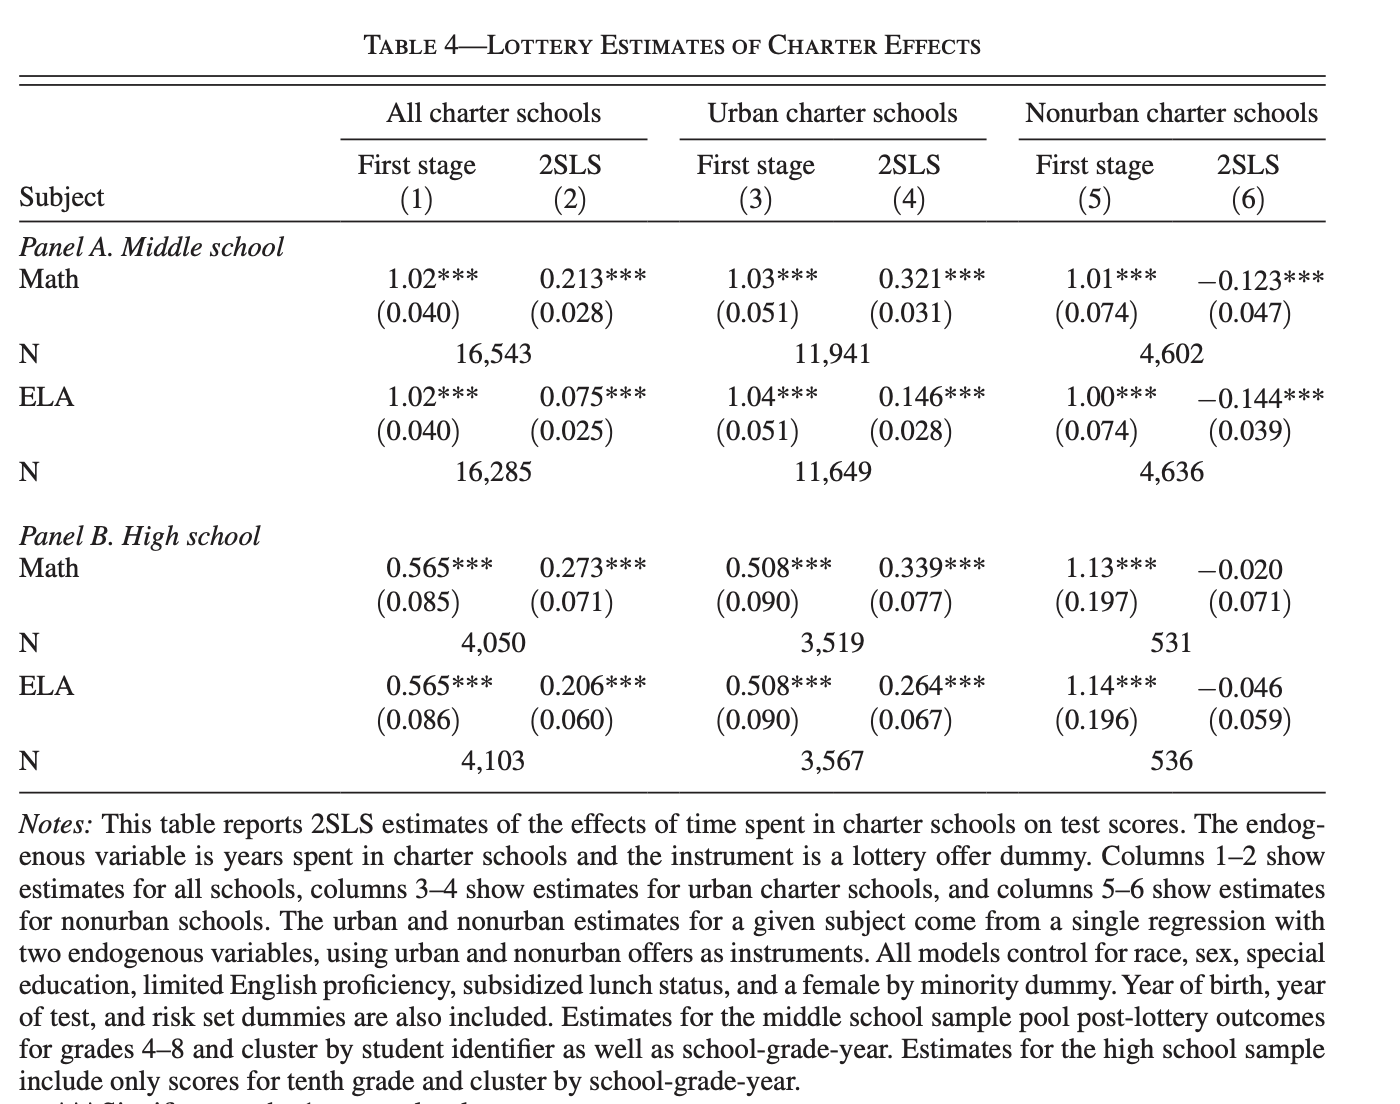
\includegraphics[width=4.5in]{./resources/apw_3.png}
\end{figure}
\end{frame}

\begin{frame}{How does it work?}
Naive comparison (this has a selection problem):
\begin{align*}
\beta = \E[Score_i \mid \text{Attend}] - \E[Score_i \mid Z_i = \text{Not Attend}] 
\end{align*}
What we want instead is:
\begin{align*}
\tau = \frac{\E[Score_i \mid Z_i = Win] - \E[Score_i \mid Z_i = Lose]}{\probP[Attend_i \mid Z_i = Win] - \probP[Attend_i \mid Z_i = Lose]} \approx \frac{\partial Score_i}{\partial Attend_i}
\end{align*}
We learn about the average improvement in test scores for those people who attend if they win the lottery and don't attend if they lose (ie: those that apply).\\
\end{frame}

\begin{frame}{Other Lotteries}
\begin{itemize}
\item Angrist (1990): How does being a veteran affect long term earnings?
\begin{itemize}
\item Problem: People who choose to serve in military are different from those who don't.
\item Solution: Vietnam War Draft Lottery numbers. Compare similar individuals with different lottery nubmers.
\item Answer: About 15\% less over lifetime (not including service era).
\end{itemize}
\item Do longer sentences affect recitivism?
\begin{itemize}
\item Judges vary (in a predictable way) in how severe they setence for certain types of crimes
\item Compare individuals of similar age, background, and crime with strict vs lenient judges.
\end{itemize}

\end{itemize}
\end{frame}



\begin{frame}{Supply and Demand (Graddy JEP)}
    \begin{align*}
    \varepsilon_D = \frac{\E[\log Q_t \mid Z_t = \text{Rainy}] - \E[\log Q_t \mid Z_t = \text{Clear}]}{\E[\log P_t \mid Z_t = \text{Rainy}] - \E[\log P_t \mid Z_t = \text{Clear}]}
    \end{align*}
\begin{itemize}
    \item What if we had something that randomly moved around \alert{supply} but didn't affect \alert{demand}.
    \item We could use this to trace out the demand curve or estimate the elasticity
    \item Weather offshore determines how many fishing boats go out, but not how much fish people want to eat (maybe?)
\end{itemize}
\end{frame}


\begin{frame}{Supply and Demand (Graddy JEP)}
\begin{figure}
\centering
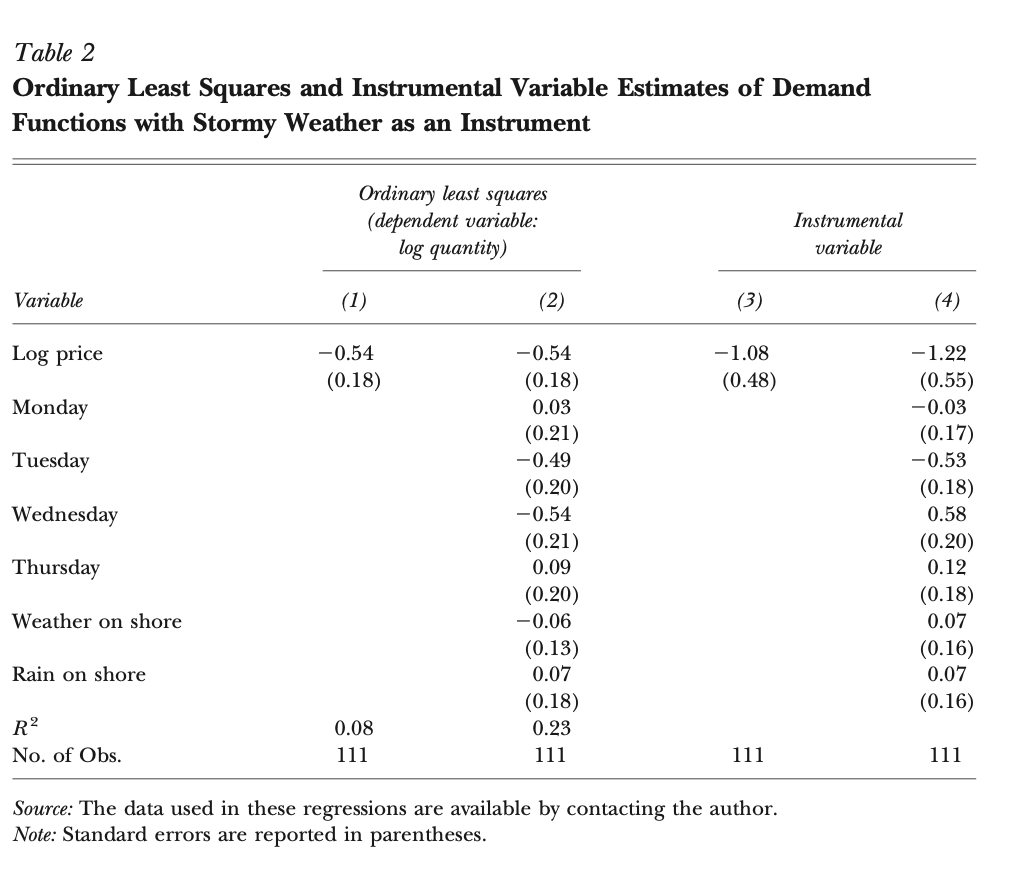
\includegraphics[height=\textheight]{./resources/graddy.png}
\end{figure}
\end{frame}


\begin{frame}{Sinkinson Starc (2021)}
Back to advertising, do ads actually work?
\begin{itemize}
\item Problem: Ad spending is often chosen as a share of revenue (oops?)
\item Problem: Ad spending is ideally chosen where it will be most effective.
\item Idea: During elections, ads for cholesterol drugs are crowded out by political ads.
\item Idea: They are crowded out even more in \alert{swing states}
\item Use this to move around the price/number of ads but not their effectiveness.
\end{itemize}
\end{frame}







\begin{frame}{Sinkinson Starc (2021)}
\begin{figure}
\centering
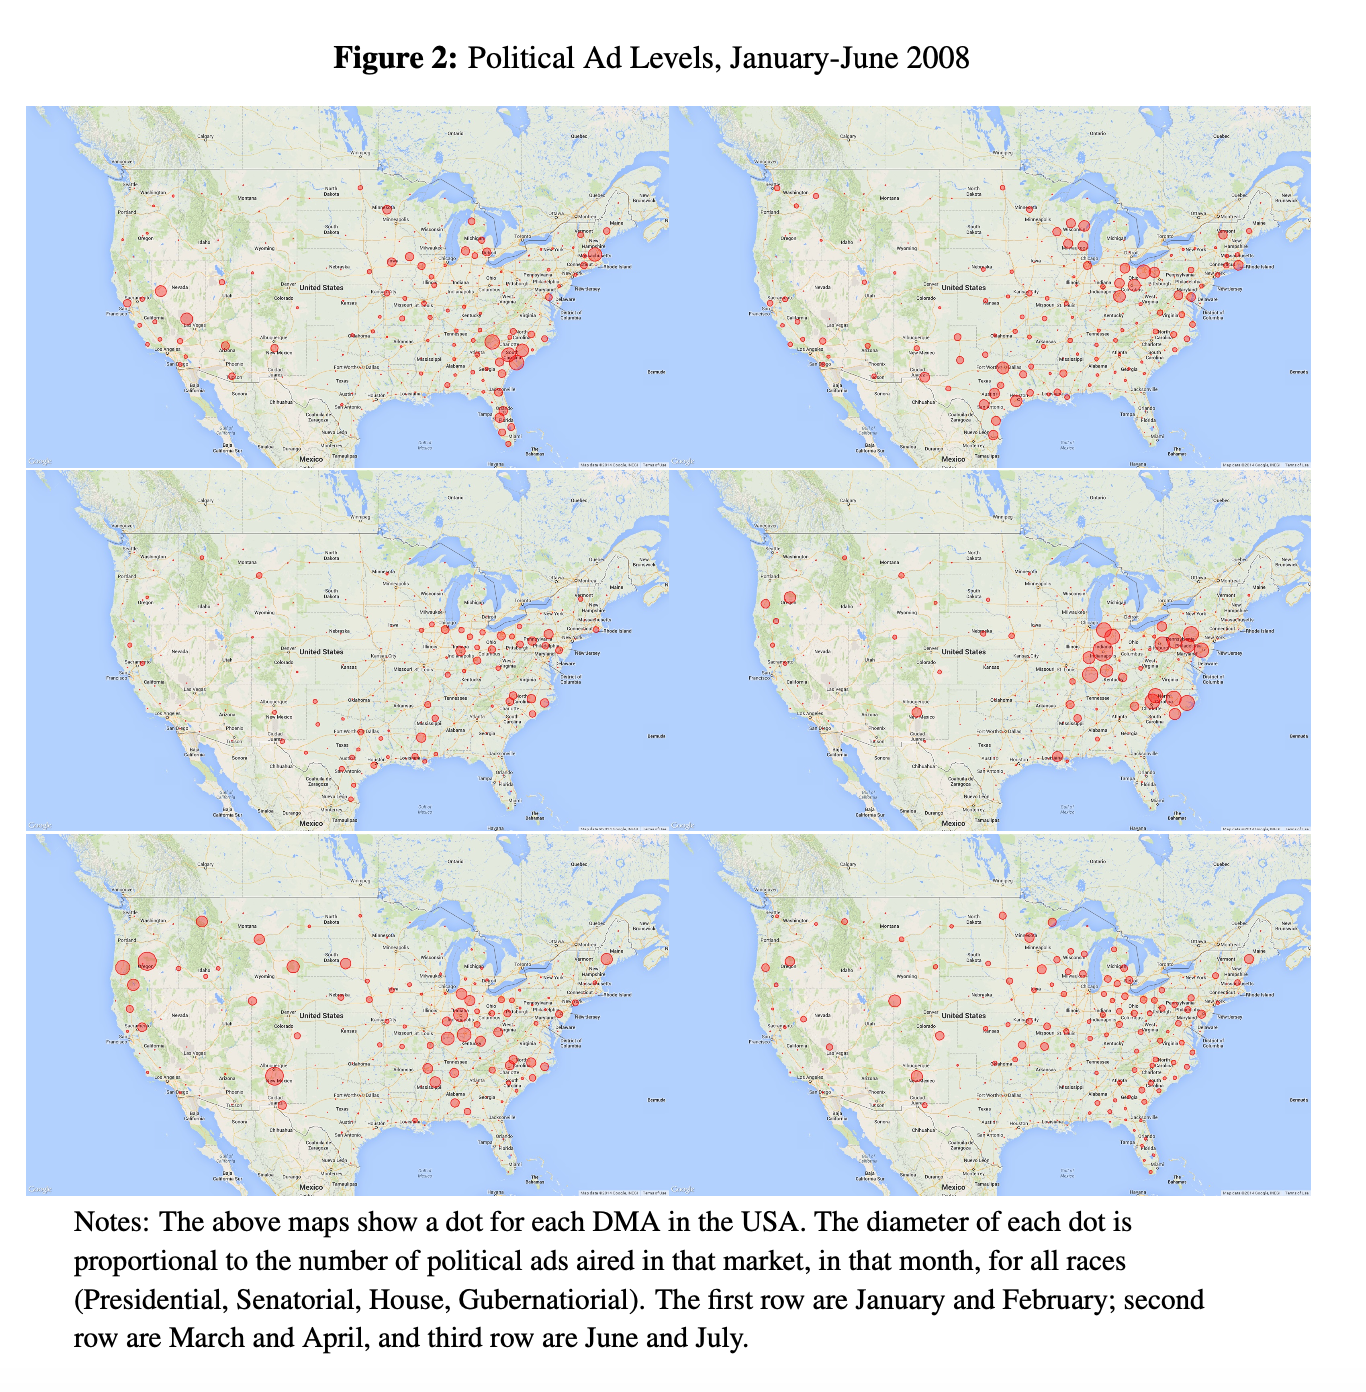
\includegraphics[height=\textheight]{./resources/ss_1.png}
\end{figure}
\end{frame}


\begin{frame}{Sinkinson Starc (2021)}
\begin{figure}
\centering
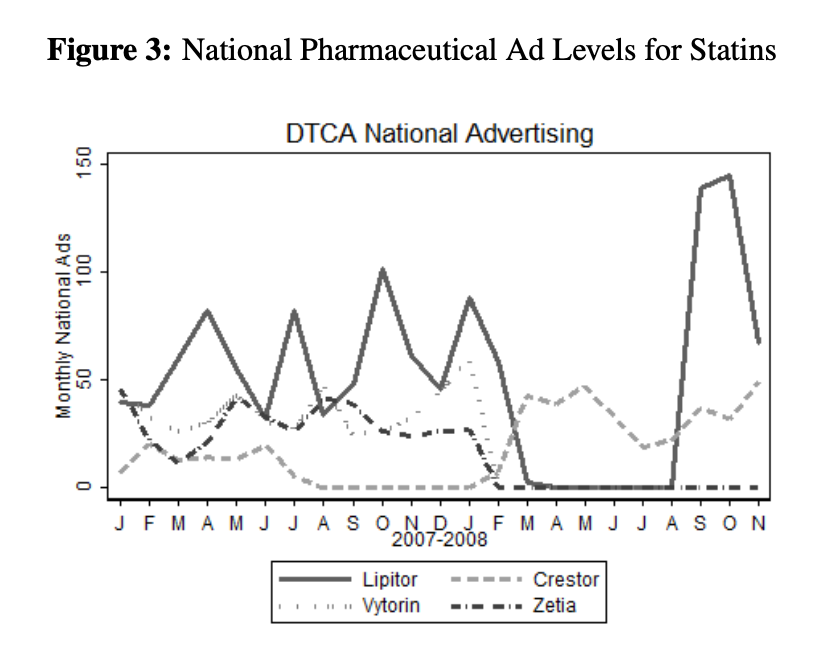
\includegraphics[height=\textheight]{./resources/ss_2.png}
\end{figure}
\end{frame}

\begin{frame}{Sinkinson Starc (2021)}
\begin{figure}
\centering
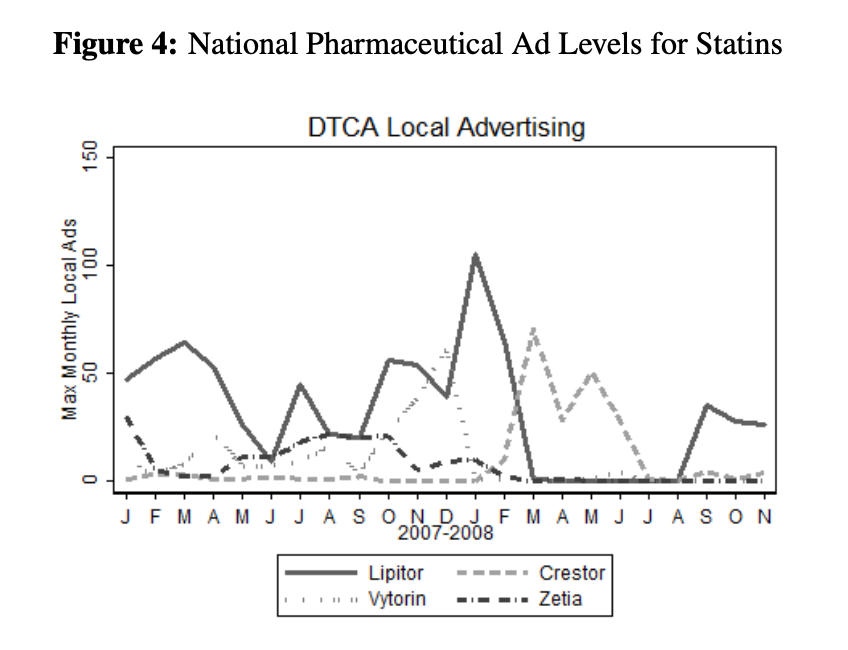
\includegraphics[height=\textheight]{./resources/ss_3.png}
\end{figure}
\end{frame}

\begin{frame}{Sinkinson Starc (2021)}
\begin{figure}
\centering
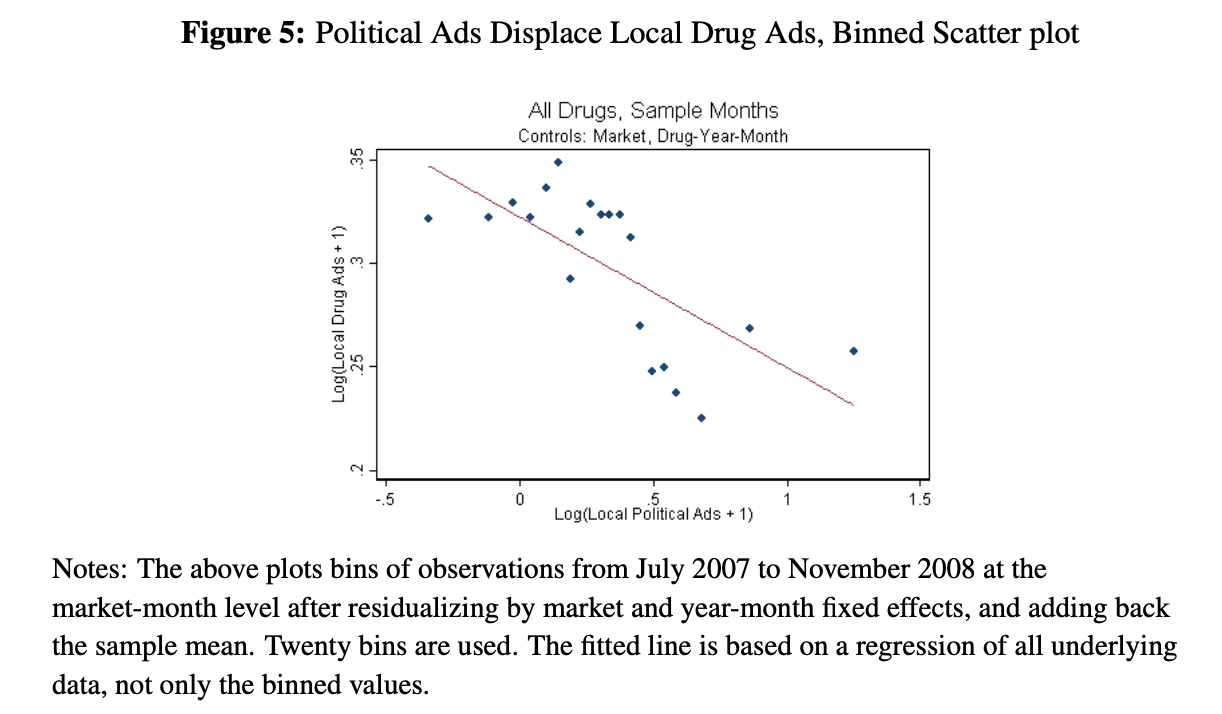
\includegraphics[height=\textheight]{./resources/ss_4.png}
\end{figure}
\end{frame}

\begin{frame}{Sinkinson Starc (2021)}
\begin{figure}
\centering
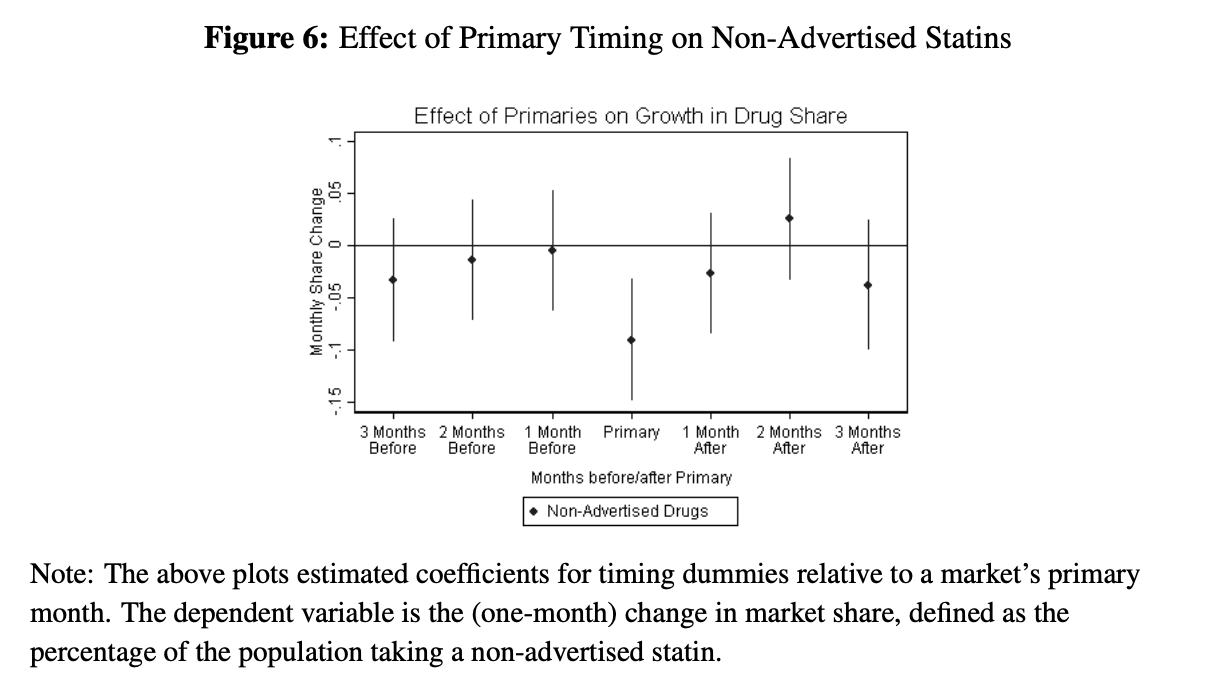
\includegraphics[height=\textheight]{./resources/ss_5.png}
\end{figure}
\end{frame}

\begin{frame}{Sinkinson Starc (2021)}
\begin{figure}
\centering
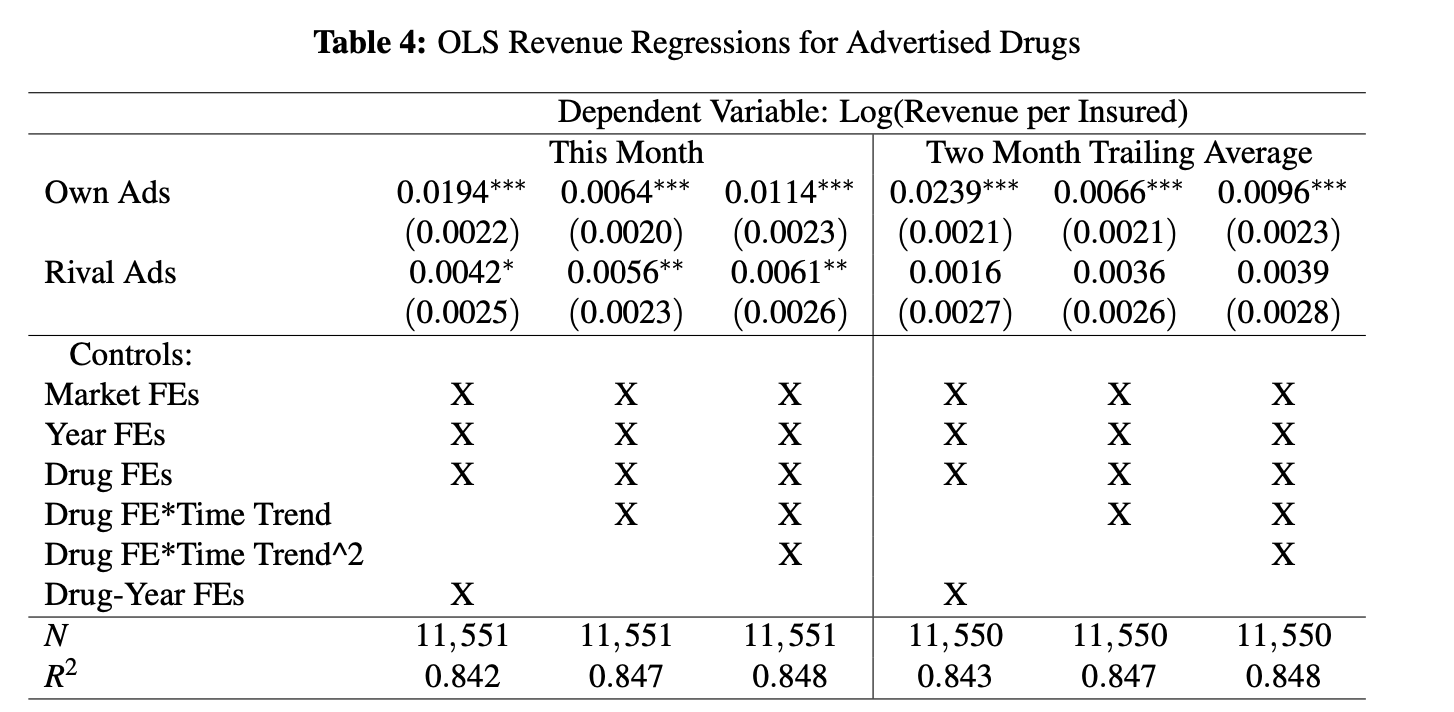
\includegraphics[width=0.9\textwidth]{./resources/ss_7.png}
\end{figure}
\end{frame}


\begin{frame}{Sinkinson Starc (2021)}
\begin{figure}
\centering
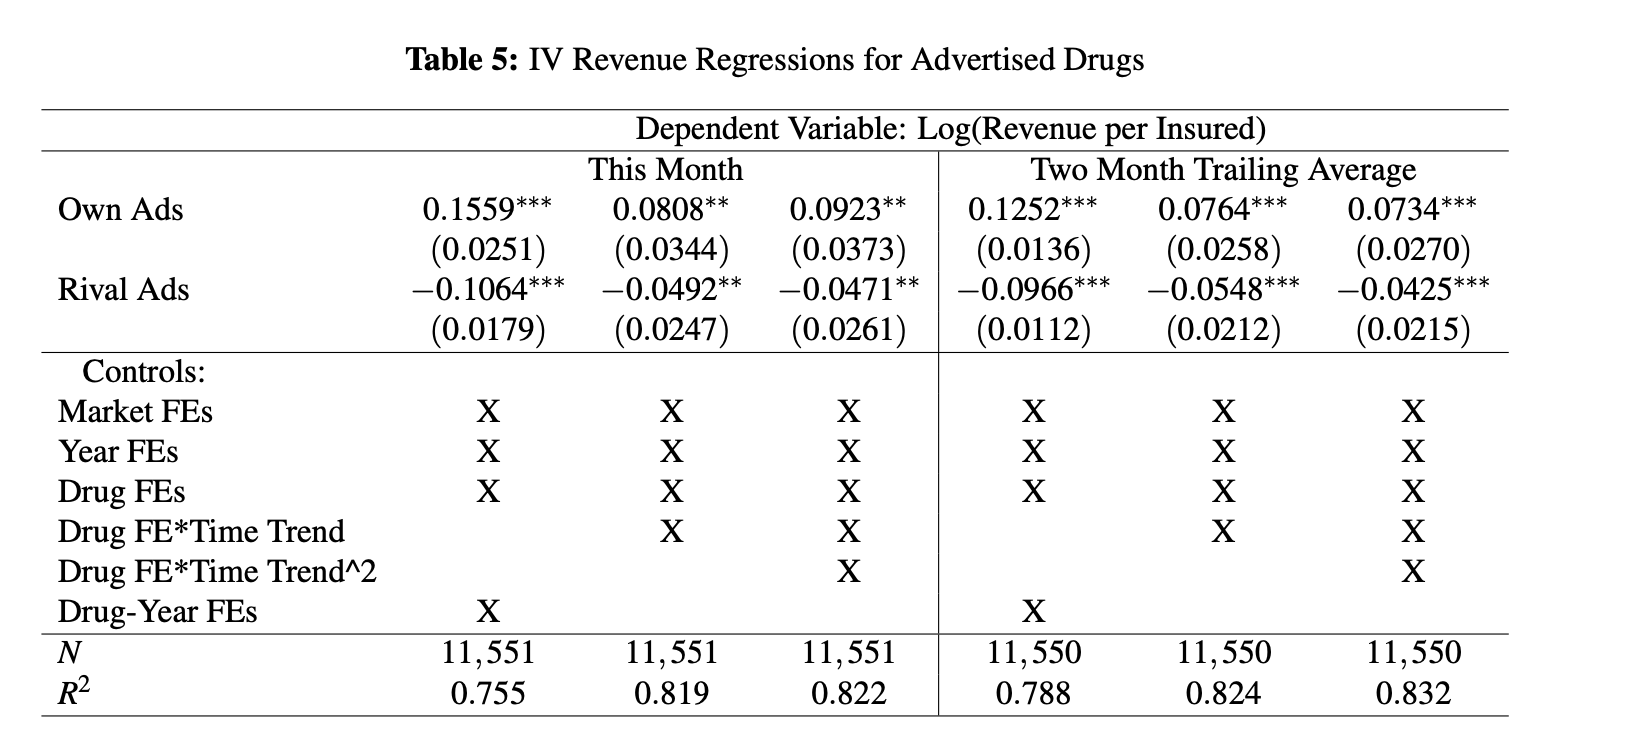
\includegraphics[width=0.9\textwidth]{./resources/ss_6.png}
\end{figure}
\end{frame}



\section{A Famous Example: Card and Krueger (AER 1994)}

\begin{frame}{A Famous Example: Card and Krueger (AER 1994)}
\begin{itemize}
\item On April 1, 1992 NJ raises its minimum wage from $\$4.25\rightarrow \$5.05$ per hour.
\item Question: Econ 101 predicts this will \alert{reduce demand for low wage workers}
\begin{itemize}
\item Focus on fast food restaurants (since they pay min wage)
\item Focus on starting wage (avoid tenure, high turnover)
\end{itemize}
\item Survey 410 restaurants in NJ (treated group) and eastern PA (control group).
\item Idea: Compare \alert{change} in wages in $NJ$ to $PA$:  $\Delta_{DD} = \Delta_{NJ}- \Delta_{PA}$
\begin{itemize}
\item Wave 1: February 15-March 4, 1992
\item Wave 2: November 5 - December 31, 1992
\end{itemize}
\end{itemize}
\end{frame}

\begin{frame}{Balance Table: Covariates}
\begin{center}
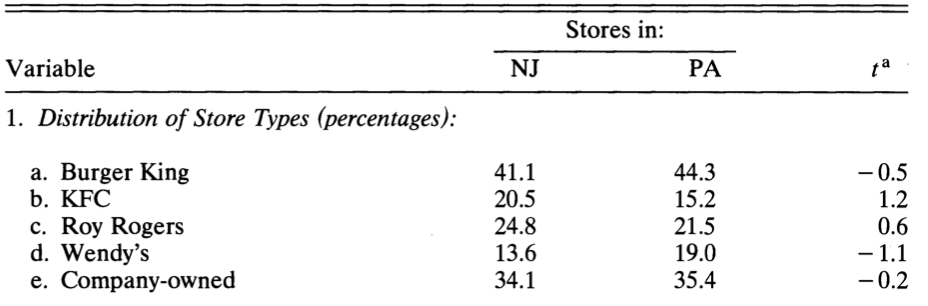
\includegraphics[width=2.25in]{./resources/ck_tab2b.png}\\
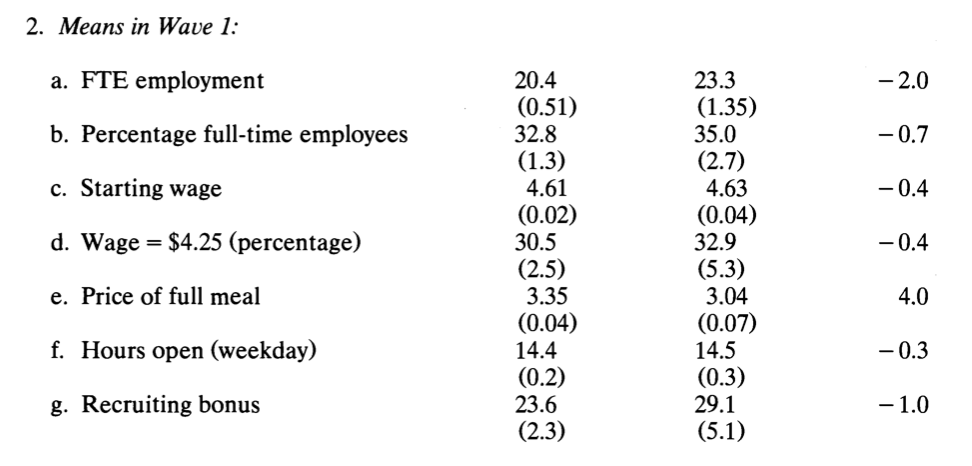
\includegraphics[width=2.25in]{./resources/ck_tab2c.png}\\
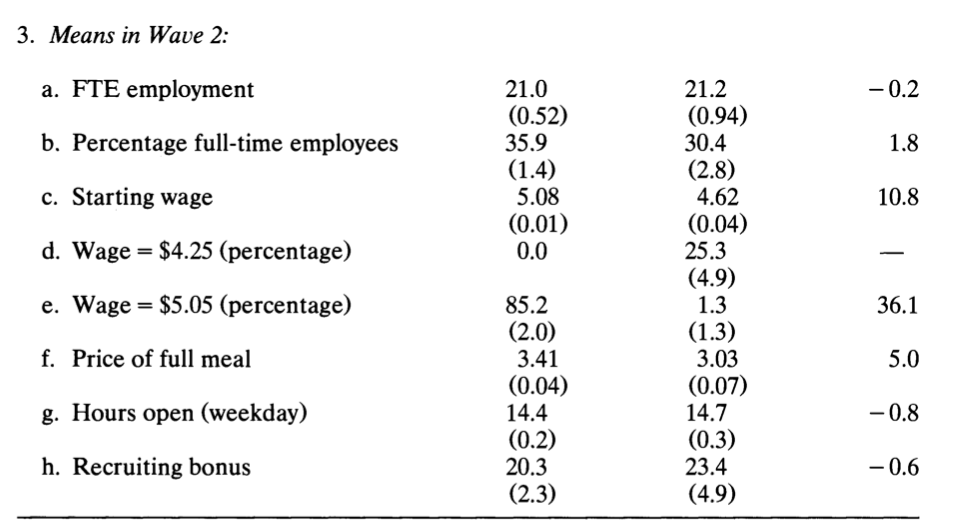
\includegraphics[width=2.25in]{./resources/ck_tab2a.png}
\end{center}
\end{frame}



\begin{frame}{Distribution of Wages}
\begin{center}
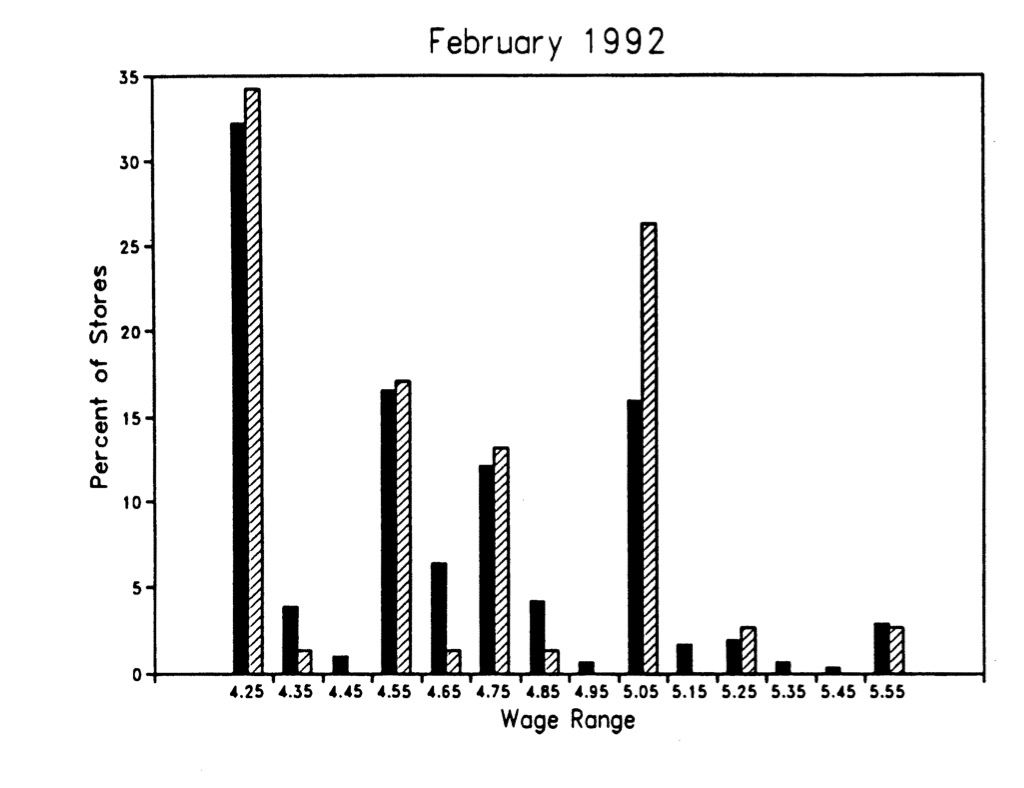
\includegraphics[width=2.75in]{./resources/ck_fig1b.png}
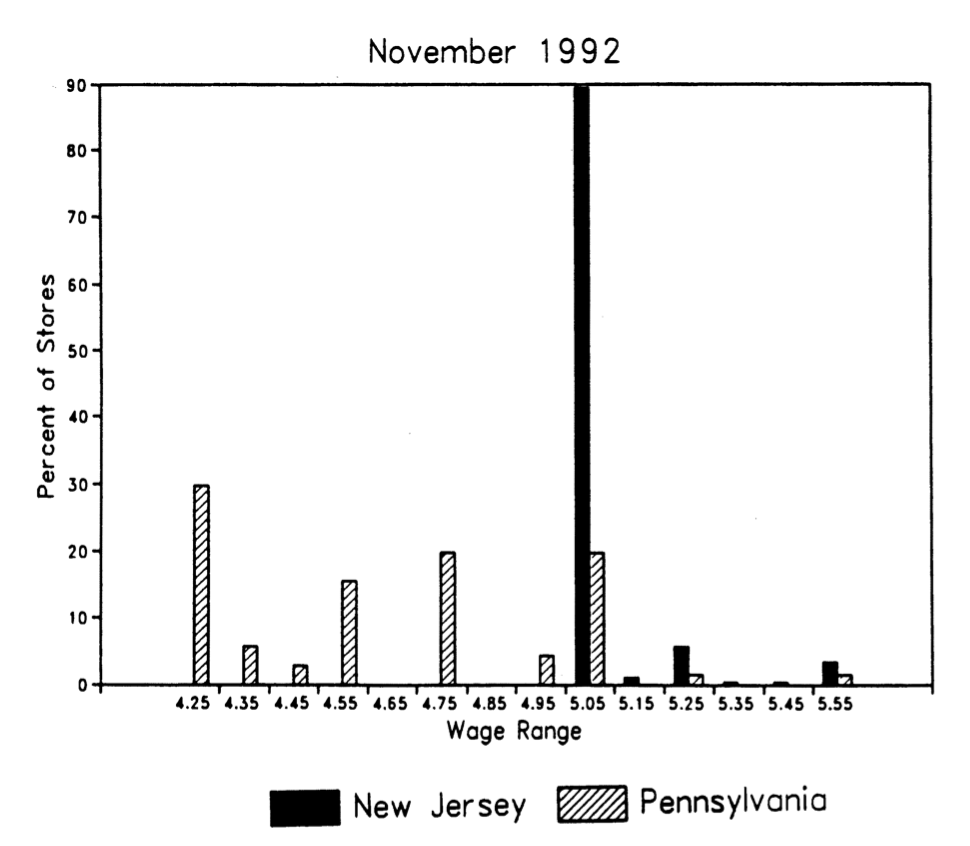
\includegraphics[width=2.5in]{./resources/ck_fig1a.png}
\end{center}
\end{frame}


\begin{frame}{Differences in Wages : 2 x 2 Table}
\begin{center}
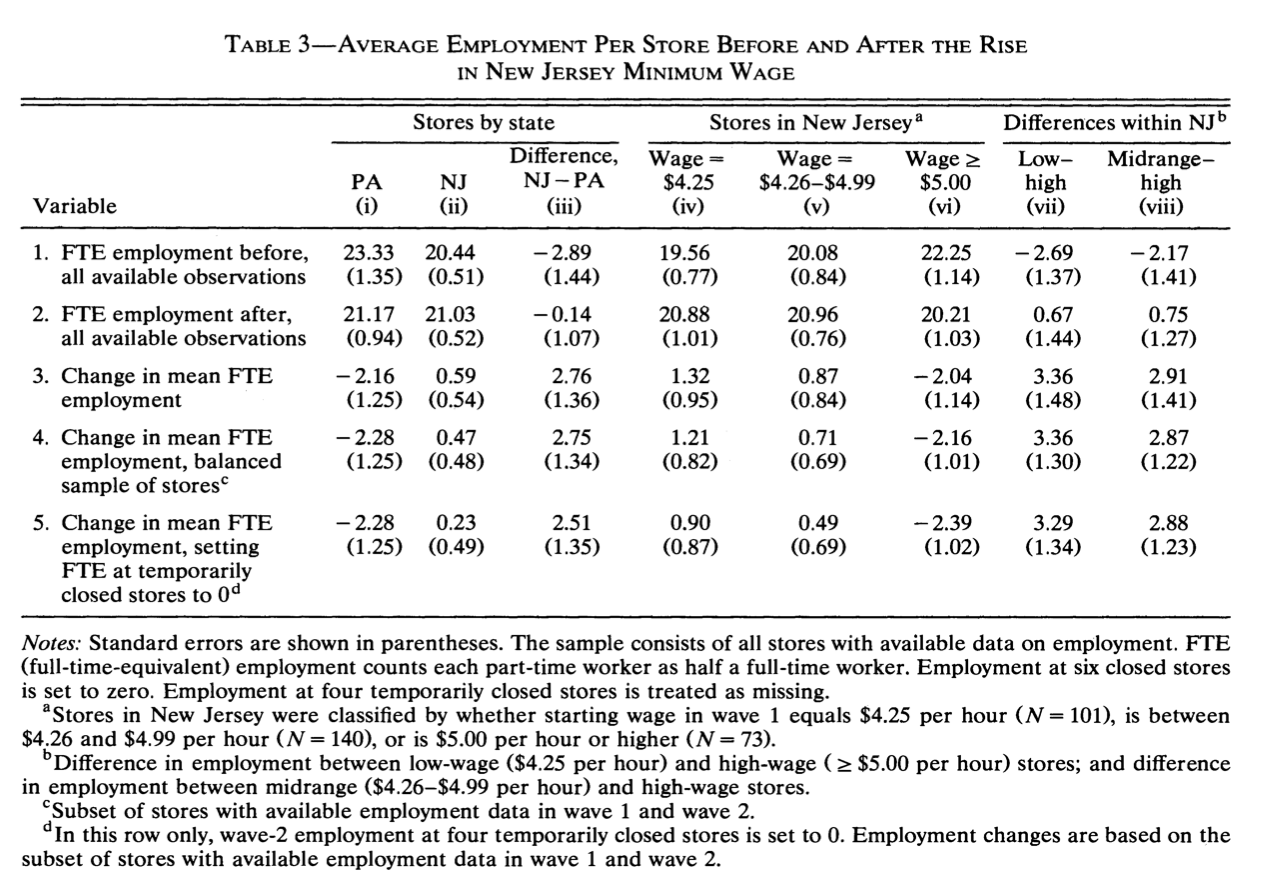
\includegraphics[width=4.25in]{./resources/ck_tab3.png}
\end{center}
\end{frame}

\begin{frame}{Outcome Equation}
\begin{itemize}
\item Differences lack any covariates (different fast food chains).
\item Also $\Delta_{PA}<0$ and $\Delta_{NJ} > 0$ (!)
\item Recall $i$ denotes stores, $t \in {1,2}$. Run the following regression:
\begin{align*}
Y_{it}&=\beta X_{it} +\alpha \cdot [i \in \text{NJ}] +  \gamma \cdot \text{After}_{t}  + \delta \cdot NJ_i \times After_{t} +u_{i}\\
Y_{it}&=\beta X_{it} +\alpha \cdot [\text{wage gap}_{i}] +  \gamma \cdot \text{After}_{t}  + \delta \cdot \text{wage gap}_{i} \times After_{t} +u_{i}
\end{align*}
\item $\alpha$ is mean difference between $NJ$ and $PA$
\item $\gamma$ is mean difference between period $1$ and $2$
\item $\delta$ is the parameter of interest, the \alert{difference in difference}
\item $\text{wage gap}_{i} = [\text{min wage}_{i,2}-w_{i1} ]_{+} =\max\{0, \text{min wage}_{i,2}-w_{i1}\} $.\\
 (How much do you need to raise $t=1$ wages to achieve minimum wage in $t=2$?)
\end{itemize}
\end{frame}

\begin{frame}{Differences in Wages}
\begin{center}
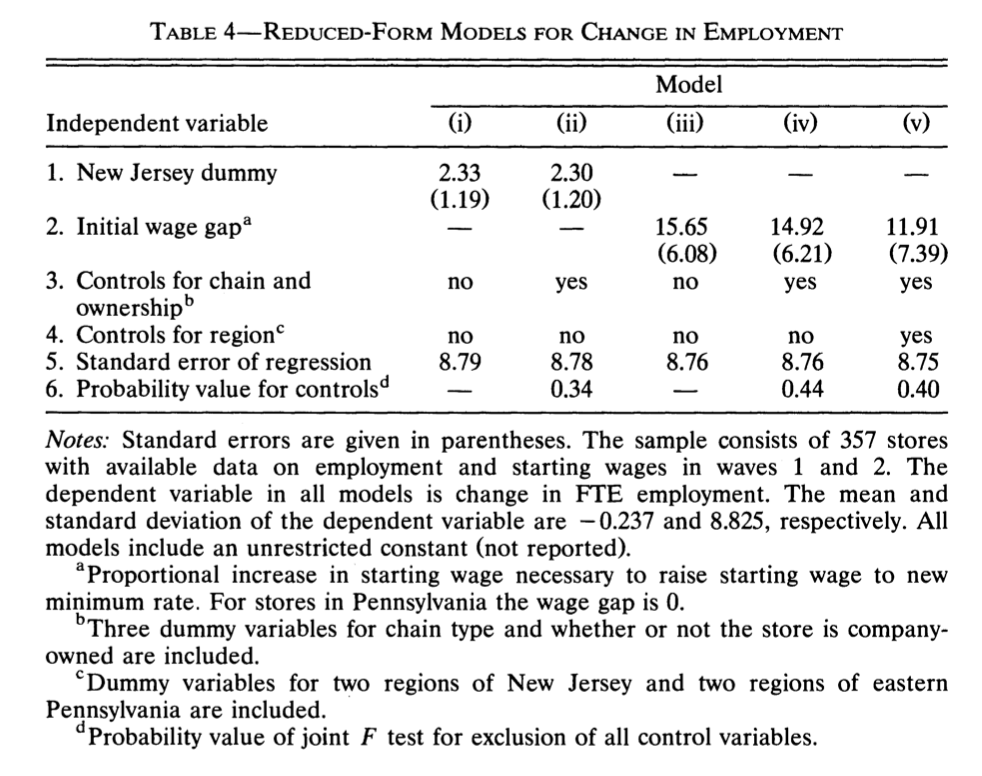
\includegraphics[width=4in]{./resources/ck_tab4.png}
\end{center}
\end{frame}


\begin{frame}{Parallel Trends}
\begin{figure}
\centering
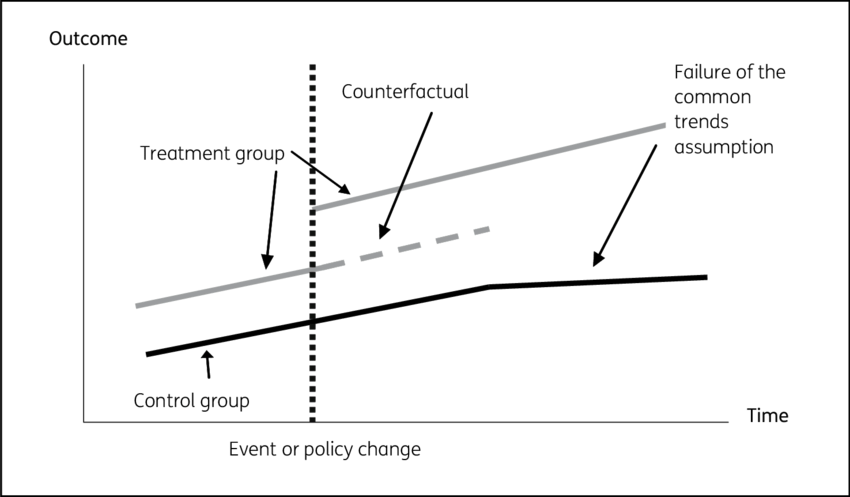
\includegraphics[width=5in]{./resources/common_trend.png}
\end{figure}
\end{frame}



\begin{frame}{Difference in Differences: Limitations}
\begin{enumerate}
\item Functional form restrictions
\begin{itemize}
\item \alert{Parallel trends} assumes that absent treatment that we add $\gamma_2 - \gamma_1$ to each unit
\item Because this is \alert{additive} it is not invariant to transformations $f(Y_{it})$ (ie: taking logs)
\end{itemize}
\item Parallel Trend Assumption is \alert{not testable}
\begin{itemize}
\item Best we can hope is that it looks similar in the pre-period
\end{itemize}
\item Compositional Effects: the treatment may affect who is in each group
\begin{itemize}
\item Restaurants could close in NJ and open nearby in PA to avoid minimum wage.
\item A good job training program may lead to migration, etc.
\item One approach: redefine the population so that it doesn't endogenously respond to treatment
\begin{itemize}
\item Recover something, but probably not ATT anymore...
\end{itemize}
\end{itemize}
\end{enumerate}

\end{frame}

\begin{frame}{Checking Pre-Trend: Card Krueger (2000)}
\begin{figure}
\centering
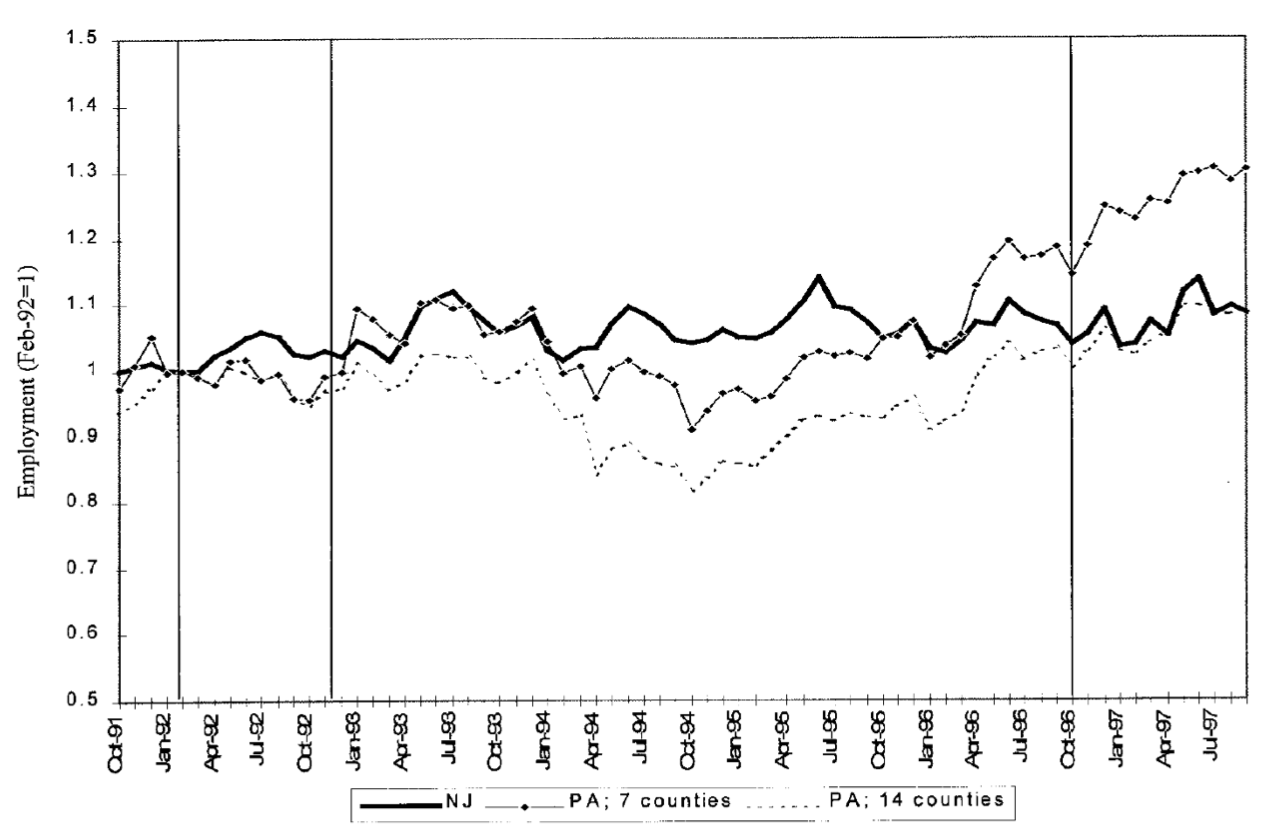
\includegraphics[width=4.5in]{./resources/card_krueger_2000.png}
\end{figure}
\end{frame}

\begin{frame}{The ``Ashenfelter Dip'' (Heckman and Smith 2000)}
\begin{figure}
\centering
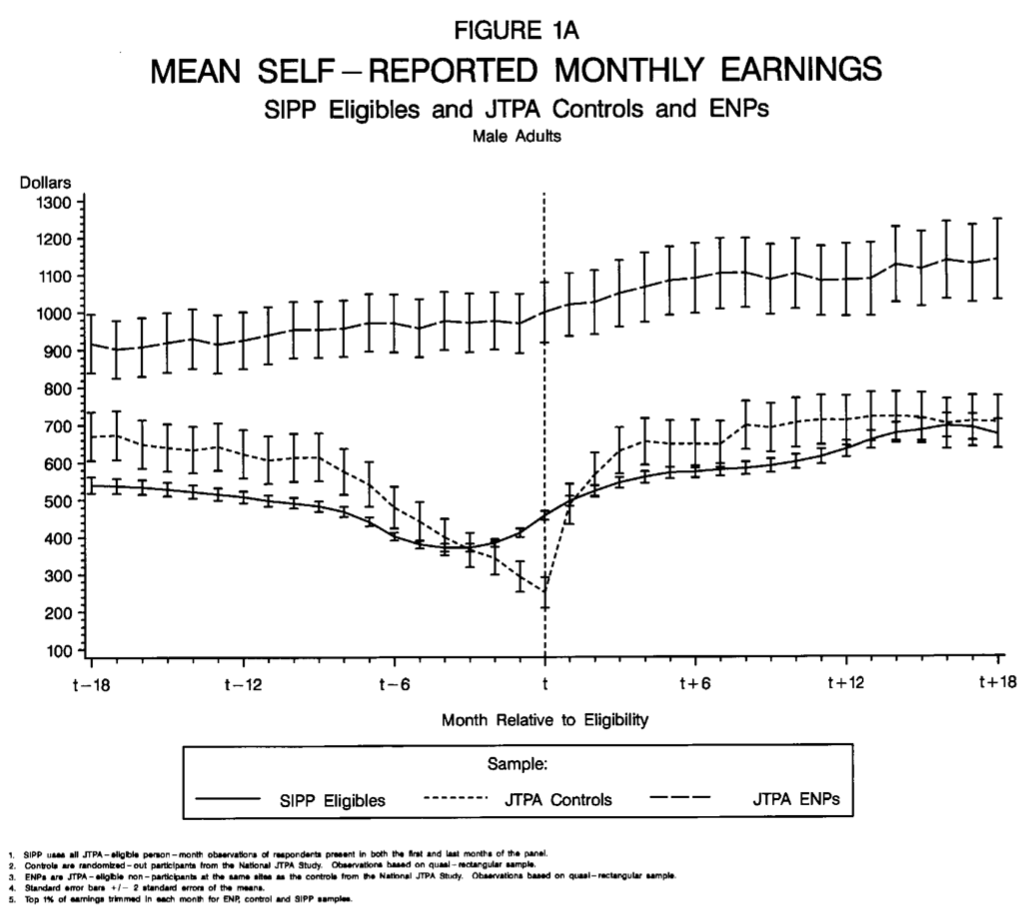
\includegraphics[width=4.25in]{./resources/ashenfelter_dip.png}
\end{figure}
\end{frame}


\begin{frame}{Motivation: Recap}
Difference in Difference approaches have some drawbacks:
\begin{itemize}
\item We need to really believe \alert{parallel trends}
\begin{itemize}
\item Is $\Delta PA$ really a good counterfactual for  $\Delta NJ$?
\item Obvious question: why not pick $\Delta DE$ or $\Delta NY$?
\item Measured effect shouldn't change if our assumption is valid (but it probably will!)
\end{itemize}
% \item With multiple treated individuals we can use 2WFE estimator
% \begin{align*}
% y_{it} = \beta X_{it} + \delta_i \cdot T_{it} +  \gamma_i + \gamma_t + u_{it}
% \end{align*}
% \vspace{-0.8cm}
% \begin{itemize}
% \item It assumes \alert{additivity} of FE $\gamma_i + \gamma_t$ are independent!
% \item States have different baseline levels $\gamma_i$ but evolution over time is common $\gamma_t$.
% \item Turns out it doesn't really generalize the diff-in-diff with $I > 2$ (Imai and Kim 2020).
% \end{itemize}            
\end{itemize}              
\end{frame}


% \begin{frame}{Motivation: Recap}
% Matching Estimators had drawbacks too:
% \begin{itemize}
% \item We need to believe in as if random-assignment conditional on $X$
% \item CIA: $\{Y_i(1), Y_i(0)\} \perp T_i | X_i$.
% \end{itemize}
% But we could use pretty flexible methods in constructing our matched controls:           
% \begin{itemize}
% \item We could try to match on multiple dimensions of $X$.
% \item $k\text{\textendash}NN$, kernels, etc.
% \end{itemize}
% What if we could use ideas from \alert{matching} to better satisfy something like our \alert{parallel trends} assumptions?
% \end{frame}

\section{Example: Abadie, Diamond, Hainmueller (2010)}

\begin{frame}{The Question}
In 1988 California passes anti-smoking Prop 99
\begin{itemize}
\item increased excise tax by 25 cents per pack, 
\item earmarked the tax revenues to health and anti-smoking education budgets and funded anti-smoking ads
\item led to indoor smoking bans in restaurants and bars city by city
\end{itemize}
 What was the effect on per capita cigarette sales?
 \begin{itemize}
 \item Already a bunch of pre-existing trends.
 \item What is a good control for California?
 \end{itemize}
 Use state-level data from 1970-2000.
\end{frame}

\begin{frame}{The Idea}
Use a convex combination of other states to construct a \alert{synthetic counterfactual California}.\\
\begin{itemize}
\item We observe $Y_{it}, X_{it},T_{it}$.
\item Assume only $i=1$ and $t > T_0$ are \alert{treated}.
\item Construct a \alert{donor pool} of potential controls subscripted by $j$.
\item Choose some \alert{weights} $w_j$ for each entity (state) in donor pool. How?
\begin{itemize}
\item Same $\mathbf{X_{1}} = \sum_j w_j \mathbf{X_{j}}$ as treated observations (like matching).
\item Same $\left({Y_{1,1},\ldots, Y_{1,T_0}} \right)= \sum_j w_j \cdot \left({Y_{j,1},\ldots, Y_{j,T_0}} \right)$ (like parallel trends).
\item Weights sum to one $\sum_j w_j = 1$ and maybe are non-negative (or not!)
\end{itemize}
\item Idea is to match all of the $X$'s and all of the $Y_{it}$'s in the \alert{pre-period}
\end{itemize}
\end{frame}

\begin{frame}{Covariate Balance}
\begin{center}
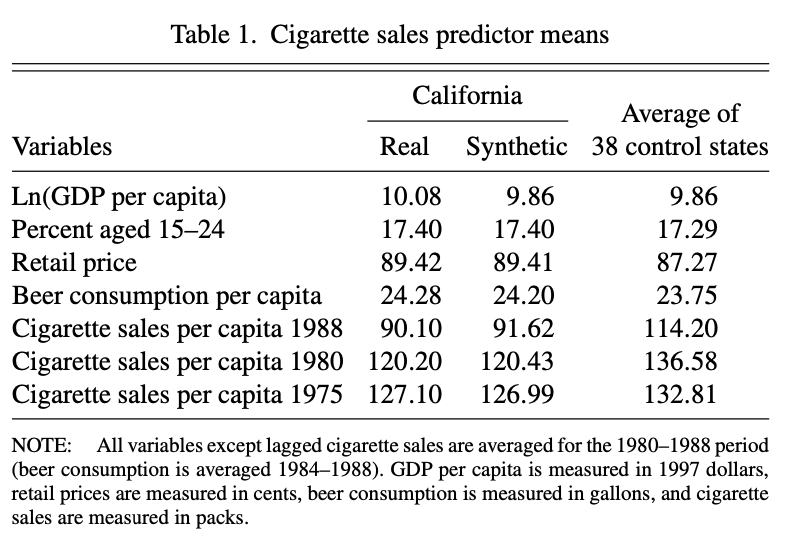
\includegraphics[width=4.5in]{./resources/abadie_1.png}
\end{center}
\end{frame}

\begin{frame}{Donor Weights}
\begin{center}
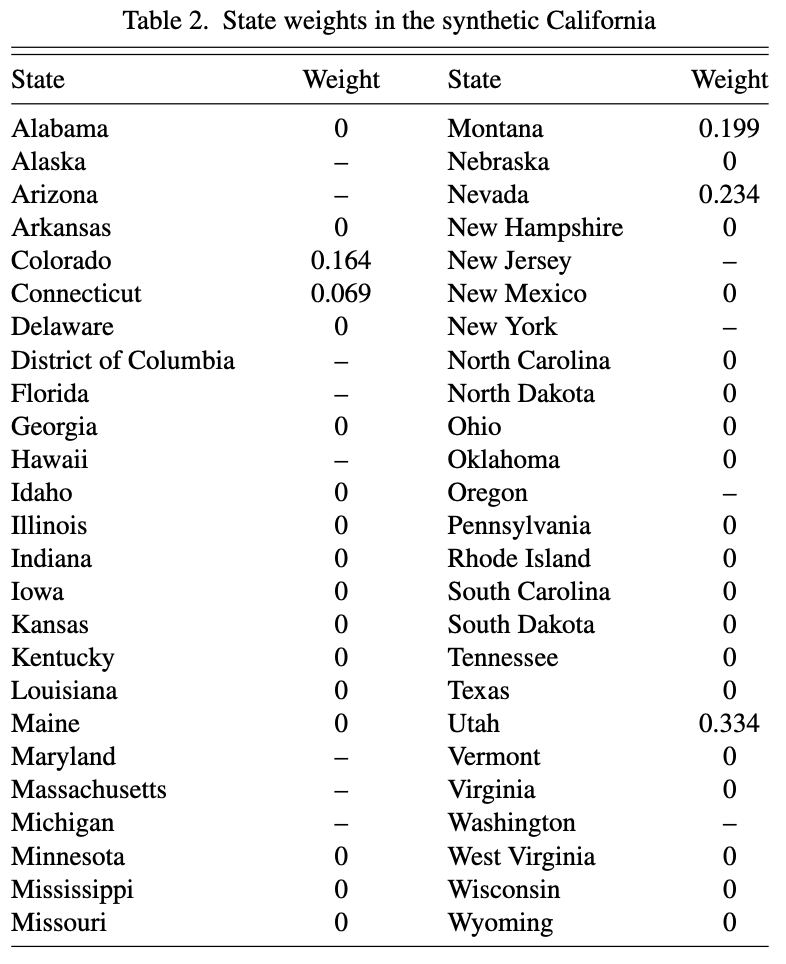
\includegraphics[width=2.5in]{./resources/abadie_2.png}
\end{center}
\end{frame}

\begin{frame}{Trend Check and Treatment Effects}
\begin{center}
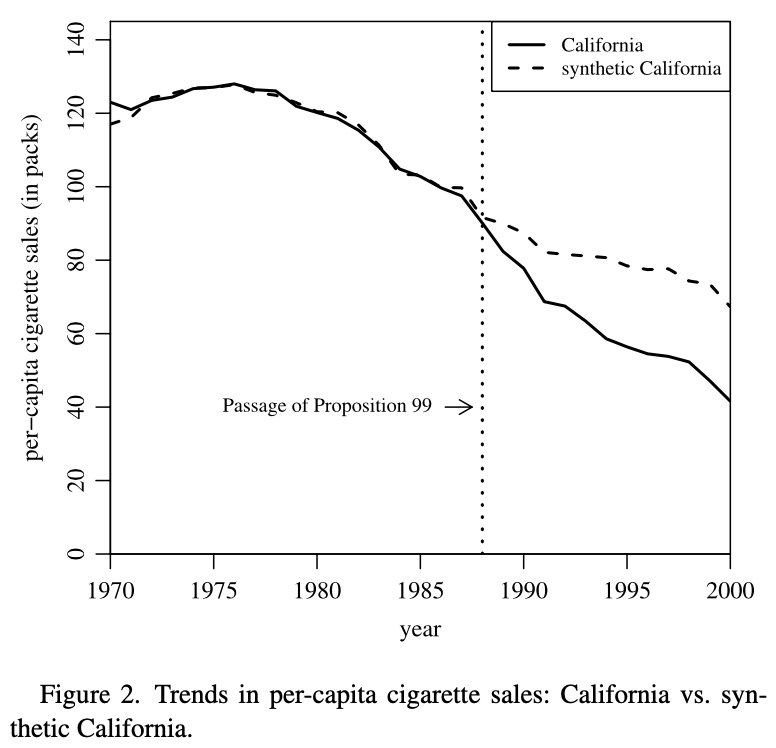
\includegraphics[width=2.75in]{./resources/abadie_3.png}
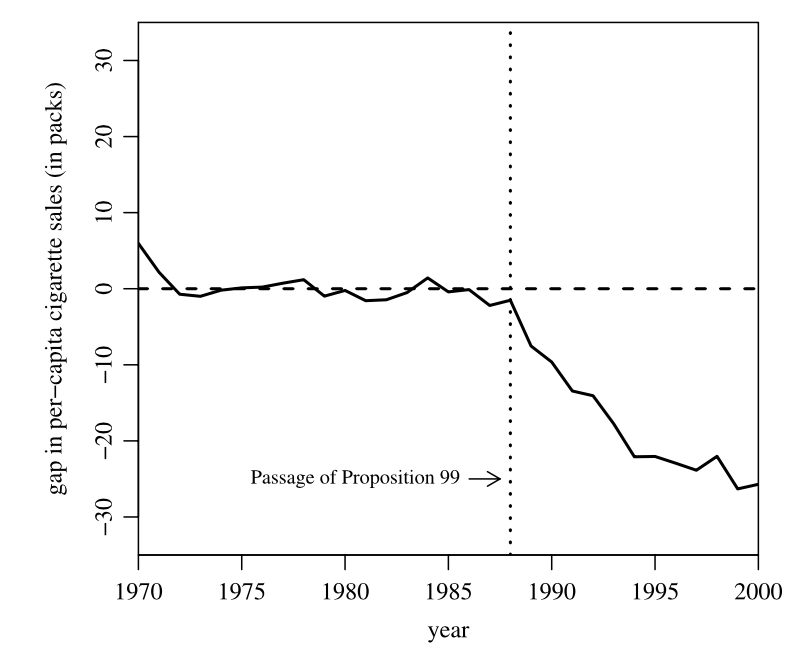
\includegraphics[width=2.75in]{./resources/abadie_4.png}
\end{center}
\end{frame}

\begin{frame}{But still some issues}
\begin{itemize}
\item How sensitive are weights estimates to different covariates?
\begin{itemize}
\item ``state-level measures of unemployment, income inequality, poverty, welfare transfers, crime rates, drug related arrest rates, cigarette taxes, population density, and numerous variables to capture the demographic, racial, and social structure of states''.
\end{itemize}
\item Can we run a \alert{placebo check}? Do we detect effects where we know there is a null effect?
\begin{itemize}
\item Put California in the donor pool.
\item Pick a state from the donor pool at pretend that receives the treatment after $T_0$
\item Choose $w_j$ following the synthetic control procedure.
\item Compute the treatment effects in the same way.
\item Repeat for all states in donor pool.
\item Compare \alert{mean-square prediction error} (MSPE) for $(Y_{1,1},\ldots,Y_{1,T_0})$
\item This doubles as \alert{inference}.
\end{itemize}
\end{itemize}
\end{frame}



\section{Regression Discontinuity Design}

\begin{frame}{Regression Discontinuity Design}
\begin{itemize}
\item Another popular research design is the \alert{Regression Discontinuity Design}.
\item In some sense this is a special case of IV regression. (RDD estimates a LATE).
\item Most of this is taken from the JEL Paper by Lee and Lemieux (2010).
\end{itemize}              
\end{frame}

\begin{frame}{RDD: Basics}
\begin{itemize}
\item We have a \alert{running or forcing variable} $x$ such that 
\begin{eqnarray*}
\lim_{x\rightarrow c^{+}} P(T_i | X_i = x) \neq \lim_{x\rightarrow c^{-}}P(T_i | X_i = x)
\end{eqnarray*}
\item The idea is that there is a \alert{discontinuous jump} in the \alert{probability of being treated}.
\item For now we focus on the \alert{sharp discontinuity}:\\
 $P(T_i | X_i \geq c) =1$ and $P(T_i | X_i < c) =0$
 \item There is no single $x$ for which we observe treatment and control.\\
  % (Compare to Propensity Score!).
\end{itemize}              
\end{frame}


\begin{frame}{RDD: Basics}
\begin{itemize}
\item Example: a social program is available to people who earned less than \$25,000.
\begin{itemize}              
\item If we could compare people earning \$24,999 to people earning \$25,001 we would have as-if random assignment. (MAYBE)
\item But we might not have that many people...
\end{itemize}
\item We are going to label the \alert{treatment effect} $\tau_i$.\\
Note: my lack of precision here!
\item The most important assumption is that of \alert{no manipulability} $\tau_i  \perp T_i$ in some neighborhood of $c$.
\begin{itemize}
\item If agents can \alert{choose} $x_i$ we are in trouble: underreporting income, avoiding ``possession with intent to distribute'' for drugs, etc.
\end{itemize}              
\end{itemize}              
\end{frame}


\begin{frame}{RDD: Continuity}
\begin{itemize}
\item The central idea in RDD is that of \alert{continuity}
\item We need that $E[Y(1)  | X]$ and $E[Y(0) | X]$ both be continuous at $X=c$.
\begin{itemize}
\item We expect that $Y_i = f(x_i)$ to be a smooth, continuous function of $x_i$
\item The \alert{only} departure from that is the treatment $\tau_i \cdot I(x_i \geq c)$.
\end{itemize}
\item We want to be as agnostic as possible about \alert{functional form}
\begin{itemize}
\item Don't want to restrict ourselves to $f(x_i) = \beta_0 + \beta_1 x_i$.
\item The central idea: we know $f(x_i)$ absent the treatment!
\end{itemize}   
\end{itemize}              
\end{frame}


\begin{frame}{RDD: In Pictures}
\begin{center}
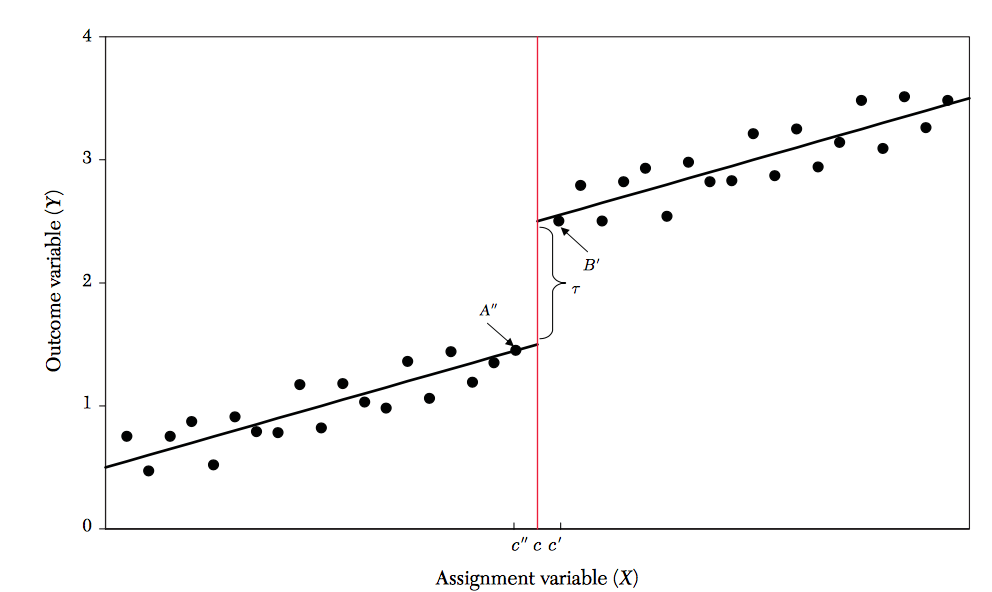
\includegraphics[width=4.5in]{./resources/ll-fig1}
\end{center}
\end{frame}


\begin{frame}{RDD: Sharp RD Case}
RDD uses a set of assumptions distinct from our LATE/IV assumptions. Instead it depends on \alert{continuity}.
\begin{itemize}
\item People just to the left of $c$ are a valid control for those just to the right of $c$.
\item \alert{This is not a testable assumption} $\rightarrow$ draw pictures!
\item We could run the regression where $T_i = \mathbf{1}[X_i > c]$.
\begin{eqnarray*}
Y_i = \beta_0 + \tau_i \cdot T_i + X_i \beta + \epsilon_i
\end{eqnarray*}
\item This puts a lot of restrictions (linearity) on the relationship between $Y$ and $X$.
\item Also (without additional assumptions) we only learn about $\tau_i$ at the point $X=c$.
\end{itemize}
\end{frame}


% \begin{frame}{RDD: Nonlinearity}
% First thing to relax is assumption of linearity.
% \begin{eqnarray*}
% Y_i = f(x_i) + \tau T_i  + \epsilon_i
% \end{eqnarray*}
% This is known as \alert{partially linear model}.
% \begin{itemize}
% \item Three options for $f(x_i)$:
% \begin{enumerate}
% \item Kernels
% \item Polynomials: $Y_i = \beta_0 + \beta_1 x_i + \beta_2 x_i^2 + \cdots + \beta_p x^p + \tau T_i + \epsilon_i$.
% \begin{itemize}
% \item Actually, people suggest different polynomials on each side of cutoff! (Interact everything with $T_i$).
% \end{itemize}
% \item Local Linear/Polynomial Regression
% \end{enumerate}
% \item Same objective. Want to flexibly capture what happens on both sides of cutoff.
% \item Otherwise risk confusing nonlinearity with discontinuity!
% \end{itemize}
% \end{frame}


\begin{frame}{Application: Lee (2008)}
Looked at incumbency advantage in the US House of Representatives
\begin{itemize}
\item Running variable was vote share in previous election
\begin{itemize}
\item Problem of naive approach: good candidates get lots of votes!
\item Compare outcomes of districts with barely $D$ to barely $R$.
\end{itemize}
\item First we plot bin-scatter plots and quartic (from each side) polynomials.
\item Discussion about how to choose bin-scatter bandwidth (CV).
\end{itemize}
\end{frame}

\begin{frame}{Lee (2008)}
\begin{center}
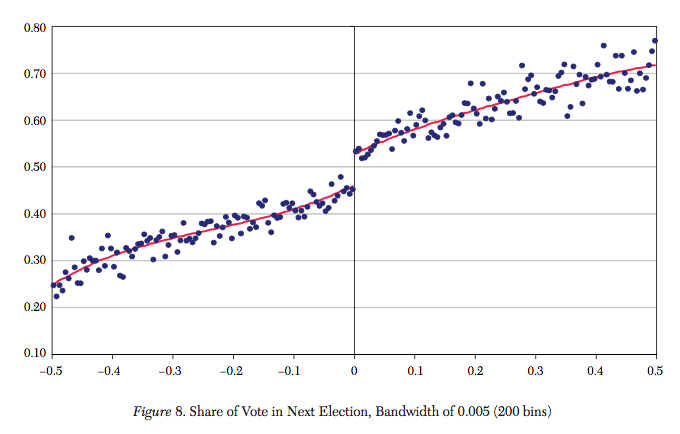
\includegraphics[width=4.5in]{./resources/binscatter1}
\end{center}
\end{frame}

\begin{frame}{Lee (2008)}
\begin{center}
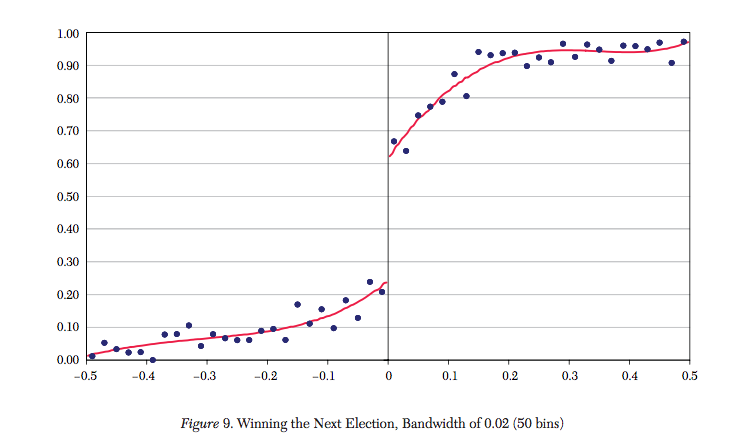
\includegraphics[width=4.5in]{./resources/binscatter2}
\end{center}
\end{frame}

\begin{frame}{Lee (2008)}
\begin{center}
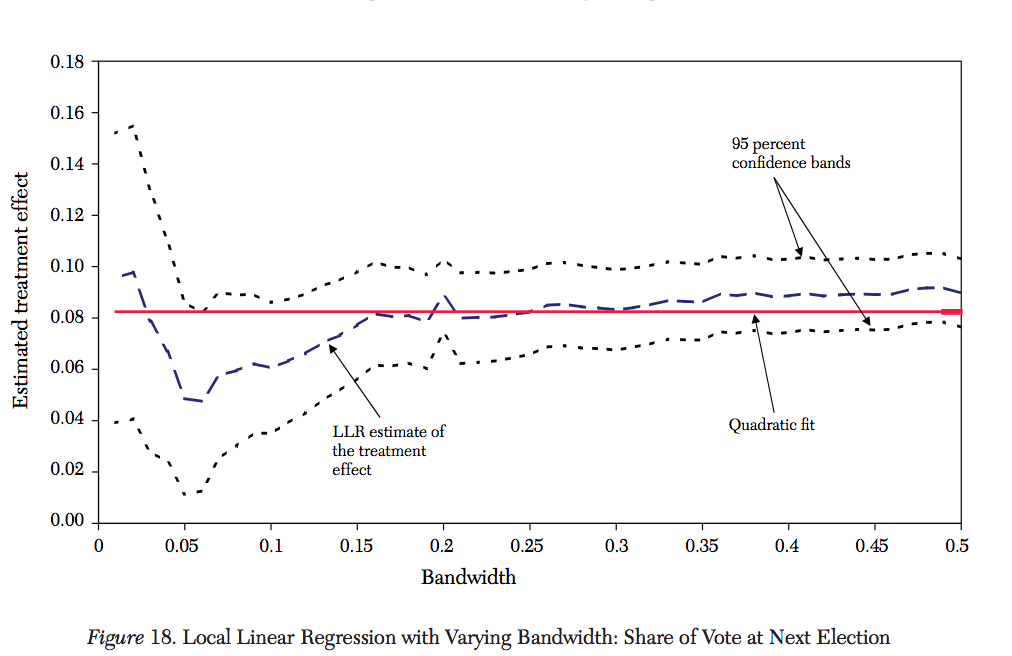
\includegraphics[width=4.5in]{./resources/ll-fig4}
\end{center}
\end{frame}

\begin{frame}{Other Examples}
Luca on Yelp
\begin{itemize}
\item Have data on restaurant revenues and yelp ratings.
\item Yelp produces a yelp score (weighted average rating) to two decimals ie: $4.32$.
\item Score gets rounded to nearest half star
\item Compare $4.24$ to $4.26$ to see the impact of an extra half star.
\item Now there are multiple discontinuities: Pool  them? Estimate multiple effects?
\end{itemize}
\end{frame}


\begin{frame}{Final Thoughts}
Always be asking
\begin{itemize}
\item What am I trying to measure?
\item What is my endogeneity problem?
\item What plausibly random variation can I use?
\end{itemize}
We don't want to look for our keys where the light is on, but you could do a lot worse than following one the scripts above !
\end{frame}




\end{document}

